\section{Einleitung}
Diese Dokument stellt die Dokumentation des Projekts \emph{Raspberry PI Security Application}, in weiterer Folge \emph{RPISec} genannt, dar, welches für die Lehrveranstaltung \emph{Mobile und ubiquitäre Systeme} realisiert wurde. In diesem Projekt wird eine Heimsicherheitsanwendung mit einem \emph{Raspberry PI 3 Model B}, \emph{Docker} und \emph{Spring Boot Microservice} umgesetzt, das bei einem Sicherheitsverstoß in der Lage ist, bekannte mobile Endgeräte von registrierten Benutzern über diesen Sicherheitsverstoß zu informieren. 

\subsection{Problemdarstellung}
Dieser Abschnitt behandelt die Problemdarstellung, welche die Grundlage für das umzusetzende Projekt \emph{RPISec} ist. Bei einem Auslösen des am \emph{Raspberry PI} angeschlossenen Bewegungssensors sollen alle am System registrierten Benutzer über ihre mobilen Endgeräte wie Handy oder Tablet über den Vorfall informiert werden, sowie die Möglichkeit haben ein Bild zu erhalten, welches den Sicherheitsbereich zum Zeitpunkt des Sicherheitsverstoßes zeigt. 
\newline
\newline
Da es sich um eine Sicherheitsanwendung handelt, soll die Benutzerverwaltung sowie die Authentifizierung \emph{In-House} gehalten werden, also die Sicherheitsanwendung selbst soll in der Lage sein die Benutzer zu verwalten und die Authentifizierungen der Benutzer durchzuführen. Da sich die mobilen Endgeräte in irgendwelchen Netzen ans Internet anbinden können, wie zum Beispiel über einen Mobilfunkanbieter, Internetanbieter oder öffentlichen \emph{Hot-Spot}, wird ein \emph{Messaging} Dienst benötigt, über den die mobilen Endgeräte erreicht werden können. Dieser \emph{Messaging} Dienst muss es erlauben, dass die Benutzerverwaltung extern erfolgen kann, da wir diesen \emph{Messaging} Dienst nicht vertrauen wollen und daher den \emph{Messaging} Dienst auch nicht die Benutzerverwaltung überlassen wollen. Ebenso wird ein online Speichermedium benötigt, dass alle Bilder speichert, damit die registrierten Benutzer jederzeit darauf zugreifen können.


\subsection{Funktionsweise}
Dieser Abschnitt behandelt die Funktionsweise der Applikation \emph{RPISec}. Die Abbildung \ref{fig:image-system-structure} zeigt den Systemaufbau der \emph{RPISec} Applikation mit der involvierten Hardware und \emph{Cloud} Dienst. 
\begin{figure}[h]
	\centering
	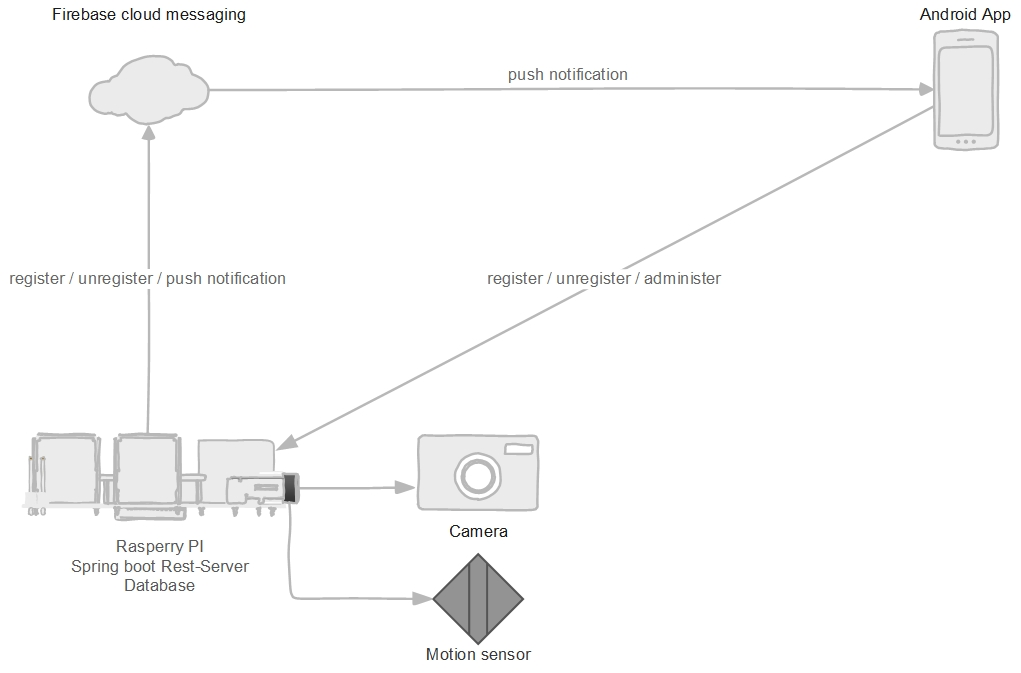
\includegraphics[scale=0.7]{\imageDir/Infrastructure.jpg}
	\caption{Systemaufbau der \emph{RPISec} Applikation}
	\label{fig:image-system-structure}
\end{figure}
\ \newpage

\subsubsection{Zugangsverifikation}
Beim Start des Systems wird vom Authentifizierungsservice \emph{(Auth-Service)} ein Administrator Benutzer erstellt, wenn dieser nicht bereits existiert. Ein neu angelegter Benutzer wird über eine E-Mail dazu aufgefordert, seinen Zugang zu aktivieren, in dem er ein Password vergibt. Im Idealfall würde die Zugangsverifikation nur im Heimnetz möglich.
\begin{figure}[h]
	\centering
	
\includegraphics[scale=0.5]{\imageDir/view-verify-account.JPG}
	\caption{Zugangsaktivierung}
	\label{fig:image-veriy-account}
\end{figure}
\begin{figure}[h]
	\centering
	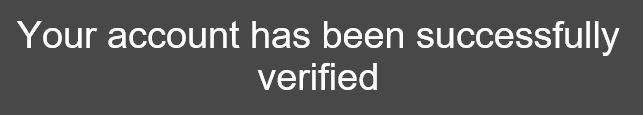
\includegraphics[scale=0.5]{\imageDir/view-verified-account.JPG}
	\caption{Bestätigung der Aktivierung}
	\label{fig:image-veriied-account}
\end{figure}

\subsubsection{\emph{Client Login}}
Die Abbildung \ref{fig:image-sequence-client-login} zeigt das Sequenzdiagramm, welches den Ablauf eines Logins eines Benutzers über einen mobilen \emph{Client} beschreibt.
\begin{figure}[h]
	\centering
	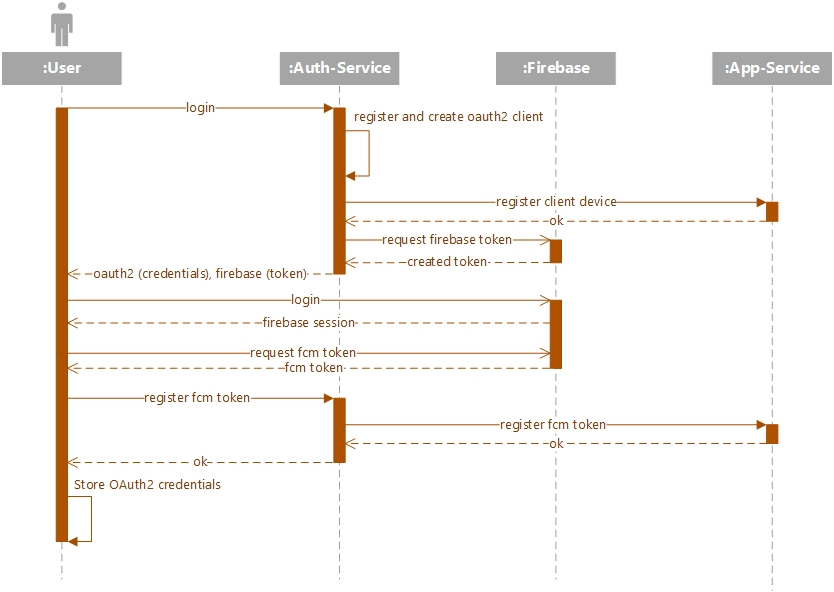
\includegraphics[scale=0.55]{\imageDir/sequence-client-login.jpg}
	\caption{Sequenzdiagramm des Logins über einen mobilen \emph{Client}}
	\label{fig:image-sequence-client-login}
\end{figure}
\ \newline
Im Zuge des Logins wird der mobile \emph{Client} am \emph{(Auth-Service)}, der die Authentifizierung durchführt, und am Applikationsservice \emph{App-Service} registriert. Der \emph{Auth-Service} erstellt bei jedem Login einen neuen \emph{OAuth2-Client} und löscht gegebenenfalls einen bestehenden  \emph{OAuth2-Client} für den mobilen \emph{Client}. Das erstellen eines \emph{OAuth2-Clients} wird durchgeführt, da mit der \emph{Client}-Applikation keine \emph{Oauth2-Client} Zugangsdaten an die mobilen \emph{Clients} mit ausgeliefert werden sollen.
\newline
\newline
Dem mobilen \emph{Client} wird bei einem Login ein \emph{Firebase} Authentifizierungstoken übermittelt, mit dem sich der \emph{Client} and \emph{Firebase} anmelden kann. Nachdem Login eines mobilen \emph{Clients} auf \emph{Firebase} holt sich der mobile \emph{Client} seine eindeutige \emph{FCM} Id in Form eines Tokens, der am \emph{Auth-Service} registriert wird, der wiederum den Token am \emph{App-Service} registriert, damit dieser in der Lage ist Nachrichten an die angemeldeten mobilen \emph{Clients} zu versenden.  

\subsubsection{Sicherheitsverstoß melden}
\begin{figure}[h]
	\centering
	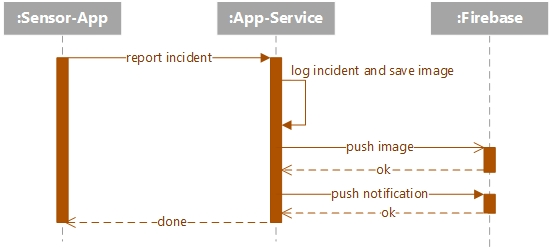
\includegraphics[scale=0.55]{\imageDir/sequence-incident.jpg}
	\caption{Sequenzdiagramm des Behandelns eines Sicherheitsverstoßes}
	\label{fig:image-sequence-incident}
\end{figure}
\ \newline
Die Abbildung \ref{fig:image-sequence-incident} zeigt das Sequenzdiagramm für das Behandeln eines Sicherheitsverstoßes, der von der Sensorapplikation erkannt und dem Applikationsservice mitgeteilt wird. Der Sicherheitsverstoß wird über \emph{Firebase} an die mobilen \emph{Clients} gemeldet, wobei einerseits eine \emph{Firebase Cloud Message (FCM)} an die mobilen \emph{Clients} versendet wird, sowie das gemachte Bild in einer \emph{Firebase} JSON-Datenbank den mobilen \emph{Clients} zum Download zur Verfügung gestellt wird. Die Benutzer können jederzeit auf die JSON-Datenbank zugreifen und sich die Bilder auf ihren jeweiligen mobilen \emph{Client} herunterladen. 
\newline
\newline
Der Ansatz einen \emph{Cloud} Dienst zu verwenden sorgt dafür, dass das \emph{RPISec} System entlastet wird, da der Datenfluss und die Netzwerkzugriffe vom System ins Internet sowie umgekehrt minimiert wird. Die Daten müssen nur einmalig in die \emph{Cloud} hochgeladen werden und die Benutzer können jederzeit, beliebig oft und von jedem beliebigen mobilen \emph{Client} darauf zugreifen.
\newpage
 
\subsubsection{\emph{Client} Nachrichtenempfang}
Die Abbildung \ref{fig:image-sequence-client-notification} zeigt den Ablauf einer  Benachrichtigung eines \emph{Client} über den \emph{Firebase Messaging} Dienst.
\begin{figure}[h]
	\centering
	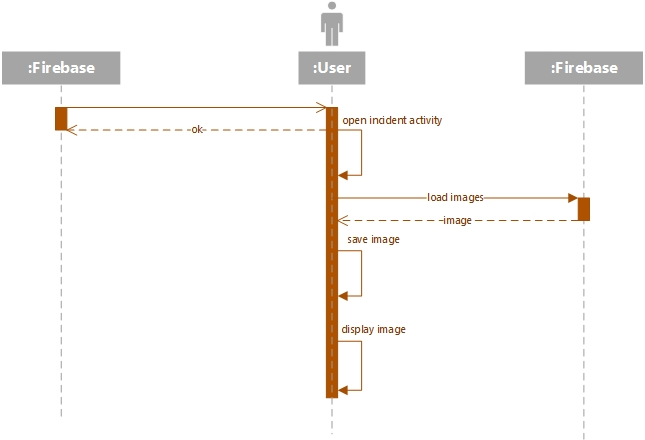
\includegraphics[scale=0.55]{\imageDir/sequence-client-notification.jpg}
	\caption{Sequenzdiagramm der Benachrichtigung eines \emph{Client}}
	\label{fig:image-sequence-client-notification}
\end{figure}
\ \newline
Nachdem das System \emph{RPISec} die mobilen \emph{Clients} via \emph{Firebase Cloud Messages} über einen Sicherheitsverstoß benachrichtigt hat, erhalten die mobilen \emph{Client}-Anwendungen die Nachricht von \emph{Firebase} und zeigen diese an. Nachdem die Benutzer auf die Nachricht geklickt haben, wird eine \emph{Activity} für das Anzeigen der Bilder geöffnet, die alle bereits gespeicherten Bilder und das neu geladene Bild anzeigt. Diese Daten werden von der \emph{Firebase} JSON-Datenbank geladen. 